\documentclass[master=ecws,masteroption=ai]{kulemt}

\setup{title={Learning a Disease Embedding using Generalized Word2Vec Approaches.  },
  author={Milan van der Meer},
  promotor={Prof.\,dr.\ Roel Wuyts},
  assessor={Ir.\,Kn. Owsmuch\and K. Nowsrest},
  assistant={Ir.\ An~Assistent \and A.~Friend}}
% The following \setup may be removed entirely if no filing card is wanted
\setup{filingcard,
  translatedtitle=,
  udc=621.3,
  shortabstract={Here comes a very short abstract, containing no more than 500
    words. \LaTeX\ commands can be used here. Blank lines (or the command
    \texttt{\string\pa r}) are not allowed!
    \endgraf \lipsum[2]}}
% Uncomment the next line for generating the cover page
%\setup{coverpageonly}
% Uncomment the next \setup to generate only the first pages (e.g., if you
% are a Word user.
%\setup{frontpagesonly}

% Choose the main text font (e.g., Latin Modern)
\setup{font=lm}

% If you want to include other LaTeX packages, do it here. 
\usepackage{graphicx}
\usepackage{float}
\usepackage{mathtools}

% Finally the hyperref package is used for pdf files.
% This can be commented out for printed versions.
\usepackage[pdfusetitle,colorlinks,plainpages=false]{hyperref}
\hypersetup{%
  colorlinks = true,
  linkcolor  = black
}


%%%%%%%
% The lipsum package is used to generate random text.
% You never need this in a real master thesis text!
\IfFileExists{lipsum.sty}%
 {\usepackage{lipsum}\setlipsumdefault{11-13}}%
 {\newcommand{\lipsum}[1][11-13]{\par And some text: lipsum ##1.\par}}
%%%%%%%

%\includeonly{chap-n}
\begin{document}

\begin{preface}
  I would like to thank everybody who kept me busy the last year,
  especially my promotor and my assistants. I would also like to thank the
  jury for reading the text. My sincere gratitude also goes to my wive and
  the rest of my family.
\end{preface}

\tableofcontents*

\begin{abstract}
  The \texttt{abstract} environment contains a more extensive overview of
  the work. But it should be limited to one page.

  \lipsum[1]
\end{abstract}

% A list of figures and tables is optional
%\listoffigures
%\listoftables
% If you only have a few figures and tables you can use the following instead
\listoffiguresandtables
% The list of symbols is also optional.
% This list must be created manually, e.g., as follows:
\chapter{List of Abbreviations and Symbols}
\section*{Abbreviations}
\begin{flushleft}
  \renewcommand{\arraystretch}{1.1}
  \begin{tabularx}{\textwidth}{@{}p{12mm}X@{}}
    LoG   & Laplacian-of-Gaussian \\
    MSE   & Mean Square error \\
    PSNR  & Peak Signal-to-Noise ratio \\
  \end{tabularx}
\end{flushleft}
\section*{Symbols}
\begin{flushleft}
  \renewcommand{\arraystretch}{1.1}
  \begin{tabularx}{\textwidth}{@{}p{12mm}X@{}}
    42    & ``The Answer to the Ultimate Question of Life, the Universe,
            and Everything'' according to \cite{h2g2} \\
    $c$   & Speed of light \\
    $E$   & Energy \\
    $m$   & Mass \\
    $\pi$ & The number pi \\
  \end{tabularx}
\end{flushleft}

% Now comes the main text
\mainmatter

\chapter{Introduction}
\label{cha:intro}
The first contains a general introduction to the work. The goals are
defined and the modus operandi is explained.

\section{Lorem Ipsum 4--5}
\lipsum[4-5]

\section{Lorem Ipsum 6--7}
\lipsum[6-7]

%%% Local Variables: 
%%% mode: latex
%%% TeX-master: "thesis"
%%% End: 

\graphicspath{ {LiteratureStudyImages/} }


\chapter{Literature Study}
\label{cha:literatureStudy}

\section{Introduction}
In this chapter 


\section{Background Knowledge}
We assume a basic knowledge of general computer science concepts as algorithms, statistics, time complexity, linear algebra, basic graph theory, optimization, and heuristics.


	\subsection{Machine Learning}
Machine learning is a data driven approach with as goal to build a model which can be	used to make predictions or decisions. This task is done by algorithms which are able to learn models based on examples given by the designer. In machine learning there are $3$ types of problems, namely supervised learning, unsupervised learning, and reinforcement learning. \\
Supervised learning is concerned with the learning task where there are examples given with their corresponding label. Unsupervised learning is similar to supervised learning only no labels are given. We won't go into reinforcement learning. \\
We can also classify to problems according to the desired output of our model. Those main tasks consist of classification, regression, clustering, and dimension reduction.
	
	
	\subsection{Time Series Analysis}
A time series consists of data points over a certain time period. We refer to this as a sequence of states. Where a state represents a data point and can differ from a single value to more complex representations like pictures. \\
The domain of time series analysis handles around extracting information or relations from a time series. It can have different goals like forecasting, classification, or exploratory.
	
	
	\subsection{Neural Networks}
	
A neural network is a machine learning approach based on biological neural networks. 


		\subsubsection{Perceptron}

The basic component of a neural network is a perceptron. A perceptron take multiple binary inputs and has a single binary output (see figure \ref{fig:perceptron}). Each input has a corresponding real numbered weight. The output is decided on the following equation:

\begin{equation} 
output =
  \begin{cases}
    0       	& \quad \text{if } \sum_j w_jx_j \leq \text{ threshold}\\
    1  		& \quad \text{if } \text{if } \sum_j w_jx_j > \text{ threshold}\\
  \end{cases}
\end{equation}
	
\begin{figure}[H]
	\centering
	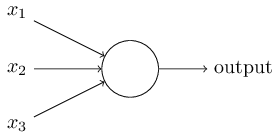
\includegraphics[width=4cm]{perceptron.png}
	\caption{A simple presentation of a perceptron.}
	\label{fig:perceptron}
\end{figure}

We can build a network by connecting multiple perceptrons (see figure \ref{fig:multiplePerceptrons}. By building these networks, more complex decisions can be made.

\begin{figure}[H]
	\centering
	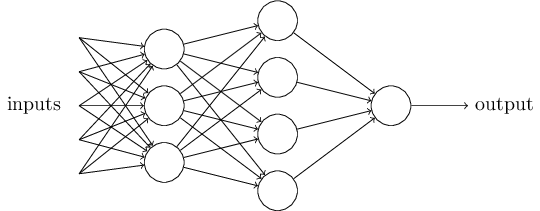
\includegraphics[width=8cm]{multiplePerceptrons.png}
	\caption{A more complex network made by connecting multiple perceptrons.}
	\label{fig:multiplePerceptrons}
\end{figure}

Now we have seen how a general network is constructed, we look at some vocabulary. \\
In figure \ref{fig:networkArch}, we see a four-layer network. As mentioned on the figure, we call the first layer the input layer, the last layer the output layer, and the layers in between are called hidden layers. Sometime multiple layer networks are referred to as multilayer perceptrons or MLPs.

\begin{figure}[H]
	\centering
	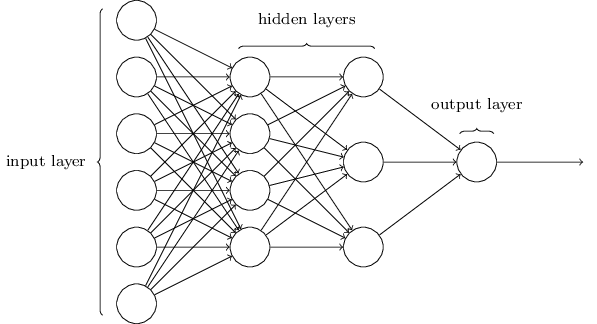
\includegraphics[width=8cm]{networkArchitecture.png}
	\caption{General vocabulary for a multilayer network.}
	\label{fig:networkArch}
\end{figure} 		


		\subsubsection{Training a network}
		
To train a neural network, we input an example with a known label. The network will have a certain output based on the current weights. When this output is incorrect, it should be possible to adjust the weights with as effect that the network now has as output the correct label. Of course, this change in weights, should only effect the output by a small bit (see figure \ref{fig:smallChange}). The reason for this is that otherwise all the previous images could now be labeled incorrectly. So, the concept of training a neural network means, adjusting the weights in a way that the behavior of the network doesn't change completely on the previous seen pictures but that the current picture is labeled correctly.

\begin{figure}[H]
	\centering
	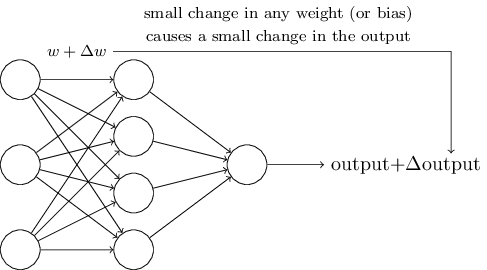
\includegraphics[width=8cm]{smallChange.png}
	\caption{A small change on the weights, only has a small impact on the output.}
	\label{fig:smallChange}
\end{figure} 

To achieve this effect, we change our known perceptrons to sigmoid neurons. A sigmoid neuron has the same basics as a perceptron. It still has inputs but now it also has a bias $b$. The inputs still have weights but the weights can now range between $0$ and $1$. The output is now calculate with $\sigma(w*x+b)$ where $\sigma$ is the sigmoid function. This results in the following formula: 

\begin{equation} 
\frac{1}{1+exp(-\sum_j w_jx_j-b)}
\end{equation}

The sigmoid function makes it possible to calculate the gradient and makes the output a linear combination of $\Delta w_j$ and $\Delta b$ as $\Delta output$ is approximated by 

\begin{equation} 
\Delta output \approx \sum_j \frac{\partial output}{\partial w_j}\Delta w_j + \frac{\partial output}{\partial b}\Delta b
\end{equation}

Because of the linearity, it is now possible to choose changes for the weights and biases to achieve a correct output. By adjusting the weights, we will train our network to achieve a higher accuracy.
		
	\subsection{Backpropagation}
	
Backpropagation is an algorithm which is used to train neural networks. It calculates the gradient of a chosen loss function with respect to the individual weights. With the gradient, the weights are updated and the loss function is minimized.

		\subsubsection{Terminology}
		
We use $w^l_{jk}$ to denote the weight corresponding to the connection between the $k^{th}$ node in the $(l-1)^{th}$ layer to the $j^{th}$ node in the $l^{th}$ layer. We use $b^l_j$ for the bias of the $j^{th}$ node in the $l^{th}$ layer and $a^l_j$ for the activation of the $j^{th}$ node in the $l^{th}$ layer. See figure \ref{fig:termNN}.

\begin{figure}[H]
	\centering
	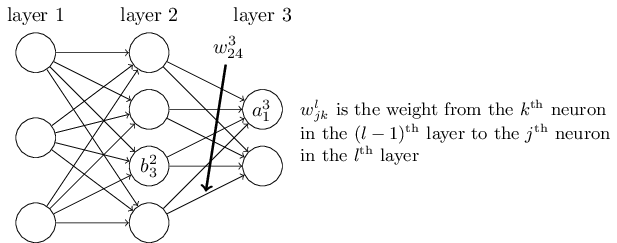
\includegraphics[width=8cm]{termNN.png}
	\caption{Visual representation of the terminology for a neural network.}
	\label{fig:termNN}
\end{figure} 

We can now convert these notation to a vector representation. We remove the indexes for the node numbers which results in the following:

\begin{equation} 
a^l = \sigma (w^la^{l-1}+b^l)
\end{equation}

		\subsubsection{Cost function}
		
AS mentioned before, backpropagation has as goal to calculate the partial derivatives of the cost function $C$ with respect to each weight and bias. \\
The cost function has to fulfill certain criteria. The first one is that it needs to be possible to write it as a summation over cost functions for individual training examples. Secondly, it needs to be derivable. And lastly, the cost function is a function of the activations of the last layer. 


		\subsubsection{Fundamental equations}

Backpropagation has 4 equations. They allow us to calculate the error for each node and adjust the weights based on the gradient descent. \\

First we calculate the error of each node which is based on how much the cost function is influenced by each activation and on how much the activation function is influenced by $z_j^L$:

\begin{equation} 
\delta^L_j = \frac{\partial C}{\partial a^L_j} \sigma'(z_j^L)
\text{ with }
z_j^L = \sum_k w^L_{jk}a^{L-1}_k+b^L_j
\end{equation}

This can be written as a neat vector equation:

\begin{equation} 
\delta^L = (a^L-y) \circ \sigma'(z_j^L)
\end{equation}

The next equation explains why the algorithm is called backpropagation. The equation calculates each layers error vector based on the layer after it, it propagates the error back over the layers:

\begin{equation} 
\delta^l = ((w^{l+1})^T\delta^{l+1}) \circ \sigma'(z_j^L)
\end{equation}

With those 2 equations we calculate the error in each layer in the neural network. Those errors can be used to calculate the derivatives of the cost function with respect to the weights and the biases:

\begin{equation} 
\frac{\partial C}{\partial w^l_{jk}} = a^{l-1}_k \delta^l_j.
\end{equation}

\begin{equation} 
\frac{\partial C}{\partial b^l_j} = \delta^l_j.
\end{equation}

When the derivatives are calculated, we can apply the gradient descent and update the weights and biases accordingly. This process represents the learning of a neural network.



http://neuralnetworksanddeeplearning.com/chap1.html


\section{Disease Progression}

\section{Word2Vec}


\section{Tsne projection}

\section{Vantage Point Tree}

\section{DeepWalk}


\section{Conclusion}
The final section of the chapter gives an overview of the important results
of this chapter. This implies that the introductory chapter and the
concluding chapter don't need a conclusion.



%%% Local Variables: 
%%% mode: latex
%%% TeX-master: "thesis"
%%% End: 

\chapter{The Next Chapter}
\label{cha:2}
\lipsum[77]

\section{The First Topic of this Chapter}
\lipsum[78]

\subsection{An item}
A master thesis is never an isolated work. This means that your text must
contain references. On-line documents\cite{wiki} as well as
books\cite{pratchett06:_good_omens} can be referenced.

\section{Figures}
Figures are used to add illustrations to the text. The \fref{fig:logo} shows
the KU~Leuven logo as an illustration.
\begin{figure}
  \centering
  
\includegraphics{logokul}
  \caption{The KU~Leuven logo.}
  \label{fig:logo}
\end{figure}

\section{Tables}
Tables are used to present data neatly arranged. A table is normally
not a spreadsheet! Compare \tref{tab:wrong} en \tref{tab:ok}: which table do
you prefer?

\begin{table}
  \centering
  \begin{tabular}{||l|lr||} \hline
    gnats     & gram      & \$13.65 \\ \cline{2-3}
              & each      & .01 \\ \hline
    gnu       & stuffed   & 92.50 \\ \cline{1-1} \cline{3-3}
    emu       &           & 33.33 \\ \hline
    armadillo & frozen    & 8.99 \\ \hline
  \end{tabular}
  \caption{A table with the wrong layout.}
  \label{tab:wrong}
\end{table}

\begin{table}
  \centering
  \begin{tabular}{@{}llr@{}} \toprule
    \multicolumn{2}{c}{Item} \\ \cmidrule(r){1-2}
    Animal    & Description & Price (\$)\\ \midrule
    Gnat      & per gram    & 13.65 \\
              & each        & 0.01 \\
    Gnu       & stuffed     & 92.50 \\
    Emu       & stuffed     & 33.33 \\
    Armadillo & frozen      & 8.99 \\ \bottomrule
  \end{tabular}
  \caption{A table with the correct layout.}
  \label{tab:ok}
\end{table}

\section{Lorem Ipsum}
This section is added to check headers and footers. So this chapter must at
least contain three pages. To make sure that we get the required amount,
the \textsf{lipsum} package isn't used but the text is put directly in the
text.

\subsection{Lorem ipsum dolor sit amet, consectetur adipiscing elit}
Sed nec tortor id felis tristique sodales. Nulla nec massa eu dui fermentum
tincidunt. Integer ullamcorper ante eget eros posuere faucibus. Nam id
ligula ut augue pulvinar vulputate id at purus. Aenean condimentum tortor
eu mi placerat eget eleifend massa mollis. Nam est mi, sagittis quis
euismod eget, sagittis in nibh. Proin elit turpis, aliquam et imperdiet
sed, volutpat eu turpis.

Pellentesque vel enim tellus, vitae egestas turpis. Praesent malesuada elit
non nisi sollicitudin non blandit lacus tincidunt. Morbi blandit urna at
lectus ornare laoreet. Suspendisse turpis diam, lobortis dictum luctus
quis, commodo at lorem. Integer lacinia convallis ultricies. Sed quis augue
neque, eu malesuada arcu. Nullam vehicula, purus vitae sagittis pulvinar,
erat eros semper massa, eu egestas nibh erat quis magna. Cras pellentesque,
nisl eu dapibus volutpat, urna augue ornare quam, quis egestas lectus nulla
a lectus.

Vivamus dictum libero in massa cursus sed vulputate eros imperdiet. Donec
lacinia, libero ac lobortis egestas, nibh dui ornare arcu, luctus porttitor
velit massa sit amet quam. Maecenas scelerisque laoreet diam, vitae congue
quam adipiscing vitae. Aliquam cursus nisl a leo convallis eleifend
fermentum massa porta. Nunc libero quam, dapibus dapibus molestie sit amet,
faucibus vel nunc.

\subsection{Praesent auctor venenatis posuere}
Sed tellus augue, molestie in pulvinar lacinia, dapibus non ipsum. Fusce
vitae mi vitae enim ullamcorper hendrerit eu malesuada est. Proin iaculis
ante sed nibh tincidunt vel interdum libero posuere. Vivamus accumsan metus
quis felis congue suscipit dapibus enim mattis. Fusce mattis tortor eget
ipsum interdum sagittis auctor id metus.

Integer diam lacus, pharetra sit amet tempor et, tristique non lorem.
Aenean auctor, nisi eu interdum fermentum, lectus massa adipiscing elit,
sed facilisis orci odio a lectus. Proin mi nibh, tempus quis porta a,
viverra quis enim. In sollicitudin egestas libero, quis viverra velit
molestie eget. Nulla rhoncus, dolor a mollis vestibulum, lacus elit semper
nisi, nec sollicitudin sem urna eu magna. Nunc sed est urna, euismod congue
mi.

\subsection{Cras vulputate ultricies venenatis}
Vivamus eros urna, sodales accumsan semper vel, lobortis sit amet mauris.
Etiam condimentum eleifend lorem, ullamcorper ornare lectus aliquet vitae.
Praesent massa enim, interdum sit amet semper et, venenatis ut elit.
Quisque faucibus, quam ac lacinia imperdiet, nulla neque elementum purus,
tempus rutrum justo massa porta sapien. Vestibulum ante ipsum primis in
faucibus orci luctus et ultrices posuere cubilia Curae; Sed ultrices
interdum mi, et rhoncus sapien rutrum sed.

Duis elit orci, molestie quis sollicitudin sed, convallis non ante.
Maecenas tincidunt condimentum justo, et ultricies leo tristique vitae.
Vestibulum quis quam non lectus dapibus eleifend a vitae nibh. Nam nibh
justo, pharetra quis iaculis consequat, elementum quis justo. Etiam mollis
lacinia lacus, nec sollicitudin urna lobortis ac. Nulla facilisi.

Proin placerat risus eleifend erat ultricies placerat. Etiam rutrum magna
nec turpis euismod consectetur. Phasellus tortor odio, lacinia imperdiet
condimentum sed, faucibus commodo erat. Phasellus sed felis id ante
placerat ultrices. Aenean tempor justo in tortor volutpat eu auctor dolor
mollis. Aenean sit amet risus urna. Morbi viverra vehicula cursus.

\subsection{Donec nibh ante, consectetur et posuere id, tempus nec arcu}
Curabitur a tellus aliquet ipsum pellentesque scelerisque. Etiam congue,
risus et volutpat rutrum, est purus dapibus leo, non cursus metus felis
eget ligula. Vivamus facilisis tristique turpis, ut pretium lectus luctus
eleifend. Fusce magna sapien, ullamcorper vitae fringilla id, euismod quis
ante.

Phasellus volutpat, nunc et pharetra semper, sem justo adipiscing mauris,
id blandit magna quam et orci. Vestibulum a erat purus, ut molestie ante.
Vestibulum ante ipsum primis in faucibus orci luctus et ultrices posuere
cubilia Curae; Proin turpis diam, consequat ut ullamcorper ut, consequat eu
orci. Sed metus risus, fringilla nec interdum vel, interdum eu nunc.
Suspendisse vel sapien orci.

\subsection{Morbi et mauris tempus purus ornare vehicula}
Mauris sit amet diam quam, eget luctus purus. Sed faucibus, risus semper
eleifend iaculis, mi turpis bibendum nisl, quis cursus nibh nisl sit amet
ipsum. Vestibulum tempor urna vitae mi auctor malesuada eget non ligula.
Nullam convallis, diam vel ultrices auctor, eros eros egestas elit, sed
accumsan arcu tortor eget leo. Vestibulum orci purus, porttitor in pharetra
eget, tincidunt eget nisl. Nullam sit amet nulla dui, facilisis vestibulum
dui.

Donec faucibus facilisis mauris ac cursus. Duis rhoncus quam sed nisi
laoreet eu scelerisque massa tincidunt. Vivamus sit amet libero nec arcu
imperdiet tempor quis non libero. Sed consequat dignissim justo. Phasellus
ullamcorper, velit quis posuere vulputate, felis erat tincidunt mauris, at
vestibulum justo lectus et turpis. Maecenas lacinia convallis euismod.
Quisque egestas fermentum sapien eu dictum. Sed nec lacus in purus dictum
consequat quis vel nisl. Fusce non urna sem. Curabitur eu diam vitae elit
accumsan blandit. Nullam fermentum nunc et leo dictum laoreet. Donec semper
varius velit vel fringilla. Vivamus eu orci nunc.

\section{Conclusion}
The final section of the chapter gives an overview of the important results
of this chapter. This implies that the introductory chapter and the
concluding chapter don't need a conclusion.

\lipsum[66]

%%% Local Variables: 
%%% mode: latex
%%% TeX-master: "thesis"
%%% End: 

% ... and so on until
\chapter{The Final Chapter}
\label{cha:n}
\lipsum[79]

\section{The First Topic of this Chapter}
\subsection{Item 1}
\subsubsection{Sub-item 1}
\lipsum[80]

\subsubsection{Sub-item 2}
\lipsum[81]

\subsection{Item 2}
\lipsum[82]

\section{The Second Topic}
\lipsum[83-85]

\section{Conclusion}
\lipsum[86-88]

%%% Local Variables: 
%%% mode: latex
%%% TeX-master: "thesis"
%%% End: 

\chapter{Conclusion}
\label{cha:conclusion}

This thesis started with explaining the new research area of Electronic Health Record Analytics. We explored the possible impact of this area as it allows to find medical patterns on a large scale. Those patterns range from drug discovery, disease progression for individuals, and reducing medical costs. At the moment several research groups are working on utilizing EHRs to find medical patterns using several methods like querying, statistics, data mining, and artificial intelligence approaches. \\
Our research sought to explore the usage of new machine learning approaches to find correlations between different diagnoses. The correlations found can be used in combination with prediction or classification methods. \\

We introduced a new way on how to apply Word2Vec methods by explaining the link between sentences of words and sequence of medical records. We call this approach a generalized Word2Vec approach and it can be applied on medical data to the correlations between different diagnoses. \\
To make sure the generalized Word2Vec methods can be applied to large-scale medical data, we applied the generalization concept also on DeepWalk. DeepWalk makes it possible to generate a smaller dataset from the original dataset and then apply a Word2Vec approach on this smaller dataset. \\
Besides the exploration on generalizing Word2Vec approaches, we also improved Word2Vec by tackling on of its shortcomings. This shortcoming of Word2Vec is that it is unable to handle unseen instances once it has built his lookup table. We combine a k-nearest neighbors method with Word2Vec and make an estimation of the correlation to other diagnoses for the unseen instance. \\

EXPERIMENTS + Limitations of the experiment

CONCLUSION

For more information about another possible experiment which also combines the Word2Vec approaches with prediction or classification methods, we refer to the next chapter. In this chapter we also talk about some possible improvements and future directions to explore.

%%% Local Variables: 
%%% mode: latex
%%% TeX-master: "thesis"
%%% End: 


% If you have appendices:
\appendixpage*          % if wanted
\appendix
\chapter{The First Appendix}
\label{app:A}
Appendices hold useful data which is not essential to understand the work
done in the master thesis. An example is a (program) source.
An appendix can also have sections as well as figures and references\cite{h2g2}.

\section{More Lorem}
\lipsum[50]

\subsection{Lorem 15--17}
\lipsum[15-17]

\subsection{Lorem 18--19}
\lipsum[18-19]

\section{Lorem 51}
\lipsum[51]

%%% Local Variables: 
%%% mode: latex
%%% TeX-master: "thesis"
%%% End: 

% ... and so on until
\chapter{De laatste bijlage}
\label{app:n}
In de bijlagen vindt men de data terug die nuttig kunnen zijn voor de
lezer, maar die niet essentieel zijn om het betoog in de normale tekst te
kunnen volgen. Voorbeelden hiervan zijn bronbestanden,
configuratie-informatie, langdradige wiskundige afleidingen, enz.

\section{Lorem 20-24}
\lipsum[20-24]

\section{Lorem 25-27}
\lipsum[25-27]

%%% Local Variables: 
%%% mode: latex
%%% TeX-master: "masterproef"
%%% End: 


\backmatter
% The bibliography comes after the appendices.
% You can replace the standard "abbrv" bibliography style by another one.
\bibliographystyle{abbrv}
\bibliography{references}

\end{document}

%%% Local Variables: 
%%% mode: latex
%%% TeX-master: t
%%% End: 
